\documentclass[12pt]{article}

\usepackage{sbc-template}

\usepackage{graphicx,url}

\usepackage[utf8]{inputenc}  
\usepackage[brazil]{babel}   

\graphicspath{ {./img/} }

\makeatletter
\def\input@path{{./sections/}}
\makeatother
     
\sloppy

\title{Estudo Comparativo de Mecanismos de Segurança Aplicados à Autenticação e Autorização em 
Sistemas Web}

\author{Rafael Strack\inst{1}, Adriano Ferrasa\inst{1}}

\address{Departamento de Informática -- Universidade Estadual de Ponta Grossa
  (UEPG)\\
  84.030-900 -- Ponta Grossa -- PR -- Brasil
\email{rafa\_strack@hotmail.com, ferrasa@uepg.br}
}
\begin{document}

\maketitle

\begin{abstract}
  This article presents a comparative study of authentication and authorization mechanisms in web
  systems, aiming to provide an in-depth analysis of the available options and their
  characteristics. The study describes the most commonly used methods such as passwords, tokens,
  multifactor authentication, and OAuth, analyzing their advantages and disadvantages. Additionally,
  sequence diagrams are provided to illustrate the usage flow of each method. Finally, a comparison
  of the studied methods is conducted, evaluating their effectiveness in terms of security. Proper
  understanding of these mechanisms is crucial to ensure the security of web systems and guide the
  correct choice in future projects.
\end{abstract}

\begin{resumo}
  Este artigo apresenta um estudo comparativo dos mecanismos de autenticação e autorização em
  sistemas web, visando fornecer uma análise aprofundada das opções disponíveis e suas
  características. O estudo descreve os métodos mais utilizados, como senhas, tokens, autenticação
  multifator e OAuth, analisando suas vantagens e desvantagens. Além disso, são apresentados
  diagramas de sequência para ilustrar o fluxo de utilização de cada método. Ao final, é
  realizada uma comparação dos métodos estudados, avaliando sua eficácia em termos de segurança. A
  compreensão adequada desses mecanismos é fundamental para garantir a segurança dos sistemas web e
  orientar a escolha correta em projetos futuros.
\end{resumo}

\section{Introdução}

Com a expansão da internet, os sistemas web assumiram um papel crucial no cotidiano de bilhões de
pessoas em todo o mundo. Desde o uso de aparelhos domésticos até o gerenciamento de 
negócios online, esses sistemas se tornaram indispensáveis para diversas atividades 
\cite{GREENGARD2015}. No entanto, a segurança desses sistemas é uma preocupação constante para 
desenvolvedores e usuários, pois há uma série de ameaças e vulnerabilidades que podem comprometer 
sua integridade.

A fundação OWASP (\emph{Open Worldwide Application Security Project}) atualiza regularmente um
relatório chamado OWASP Top 10, onde são descritos os 10 riscos de segurança mais críticos em
sistemas web. Na última edição, realizada em 2021, a categoria que ficou em primeira colocação foi
a quebra de controle de acesso. Em sétima colocação, ficou a categoria de falhas de identificação e
autenticação \cite{OWASP2021}. Esses problemas são diretamente relacionados aos processos de
autenticação e autorização de usuários, os quais são essenciais para garantir a proteção adequada
dos sistemas.

De modo geral, a autenticação é o processo de validação de usuários, enquanto a autorização é o
método que fornece as permissões de acesso corretas aos recursos para usuários previamente
autenticados \cite{TUMIN2012}. Atualmente, existem diversos mecanismos de autenticação e autorização
de usuários disponíveis, como senhas, \emph{tokens}, autenticação multifator, OAuth, OpenID, entre
outros. Cada um desses mecanismos apresenta características distintas, pontos positivos e negativos,
sendo fundamental garantir a correta implementação dos mecanismos escolhidos, de forma a assegurar
a efetividade da segurança dos sistemas web.

Diante desse contexto, o presente trabalho tem como objetivo realizar um estudo
comparativo dos diferentes mecanismos de autenticação e autorização, com o propósito
de fornecer uma análise aprofundada que auxilie na escolha adequada desses mecanismos
em projetos de sistemas web. O estudo visa oferecer uma compreensão ampla das
características, pontos fortes e limitações de cada mecanismo, permitindo a seleção
correta e a implementação eficiente das medidas de segurança necessárias.

\section{Autenticação e Autorização}

Na maioria dos sistemas \emph{web}, é necessário realizar um controle de acesso para que somente
certos usuários possam acessar recursos protegidos. Para isso, o mecanismo  de controle de
acesso depende de dois processos relacionados: a autenticação e a autorização
\cite{SULLIVAN2011}.

A autenticação pode ser definida como o processo de confirmação de identidade. Porém, em sistemas 
\emph{web}, devido a falta de conhecimento do mundo real, este processo pode não ser simples
\cite{CHAPMAN2012}. Existem três grupos de fatores amplamente utilizados para confirmar a
identidade de um usuário: algo que o usuário sabe, algo que o usuário é e algo que o usuário
possui. No primeiro grupo, inclui-se as senhas, PINs (\emph{Personal Identification Number}) e
frases secretas. No segundo grupo, inclui-se certificados digitais, \emph{smart cards} e
\emph{tokens} de segurança. O terceiro grupo inclui técnicas biométricas, como como impressões
digitais, reconhecimento facial ou de voz, entre outras \cite{SULLIVAN2011}.

De forma complementar, a autorização é o processo pelo qual o sistema verifica se um usuário 
previamente autenticado possui permissão para acessar um recurso ou executar uma determinada ação 
\cite{SPILCA2020}. Ela pode ser realizada de várias formas, porém as mais comuns são as baseadas em 
usuários, perfis (\emph{roles}) e com o uso do protocolo OAuth \cite{CHAPMAN2012}.

\subsection{Autenticação Básica HTTP}

A autenticação básica HTTP (\emph{Hypertext Transfer Protocol}) foi definida na especificação
HTTP/1.0 \cite{RFC1945}, porém tornou-se um padrão na RFC 2617 \cite{RFC2617}. Neste tipo de
autenticação, o servidor web recusa uma transação caso o cliente não esteja autenticado,
desafiando-o para obter um nome de usuário e senha válidos. Este desafio de autenticação é iniciado
retornando o status HTTP 401 (não autorizado) e especificando o domínio de segurança
(\emph{security realm}) a ser acessado, com o cabeçalho \texttt{WWW-Authenticate}. Ao receber o 
desafio, o cliente abre uma caixa de diálogo para que o usuário insira as credenciais para acesso 
ao domínio. O cliente então junta as informações de usuário e senha, colocando dois pontos entre 
eles, e os codifica usando o método de codificação base-64. Estas credenciais codificadas são 
colocadas no cabeçalho \texttt{Authorization}, e então a requisição é enviada para o servidor, que 
fará a validação das credenciais e, caso validadas, retorna-se o status HTTP 200 (OK) 
\cite{GOURLEY2002} (Figura \ref{fig:basicAuth}).

\begin{figure}[ht]
  \centering
  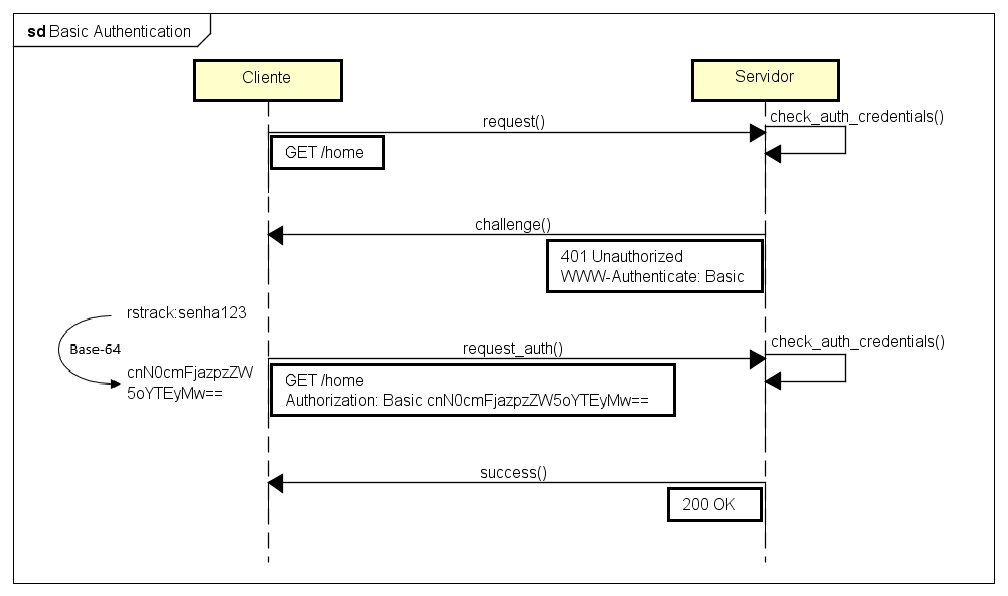
\includegraphics[width=.8\textwidth]{Basic Authentication.png}
  \caption{Exemplo de autenticação básica HTTP}
  \label{fig:basicAuth}
\end{figure}

A diretiva de domínio (\emph{realm}) utilizada nas autenticações HTTP define os espaços de proteção 
do sistema web. Esses domínios permitem que os recursos protegidos sejam particionados, cada um com 
seu próprio esquema de autenticação e/ou autorização \cite{RFC2617}.



\subsection{Autenticação \emph{Digest} HTTP}

A autenticação \emph{Digest} foi especificada na RFC 2019 \cite{RFC2019}, porém também foi 
realocada para a RFC 2617. Foi desenvolvida para ser uma alternativa mais compatível e segura  para 
a autenticação básica, corrigindo as falhas mais graves da mesma, como a falta de criptografia de 
senhas, vulnerabilidade a captura e reprodução de pacotes e proteção contra vários outros tipos 
comuns de ataques \cite{GOURLEY2002}.

Assim como a autenticação básica HTTP, a \emph{Digest} é baseada no paradigma 
desafio-resposta \cite{RFC7616}. A diferença é que foram adicionados diversos parâmetros nos 
cabeçalhos, para identificação única de desafios, nível de qualidade de proteção, especificação de 
algoritmo de hashing utilizado entre outros recursos \cite{CHAPMAN2012}. Por padrão, o algoritmo 
utilizado é o MD5, porém na RFC 7616 foram adicionados e recomendados os algoritmos SHA-256 e 
SHA-512/256 \cite{RFC7616}.

O parâmetro \texttt{response} é a principal parte do cabeçalho \texttt{Authorization}: ele contém 
uma concatenação criptografada de dados da requisição, como nome do usuário, \texttt{realm}, senha, 
método HTTP, URL, entre outros parâmetros, todos separados por dois pontos. \cite{CHAPMAN2012}. O 
cliente realiza o cálculo resultante no valor de \texttt{response}. O servidor também o faz e 
compara com o valor recebido. Caso as credenciais sejam válidas, retorna-se o status HTTP 200 (OK)
e o cabeçalho \texttt{Authentication-Info}, que contém parâmetros utilizados para uma futura 
autenticação, autenticação mútua e reenvio de parâmetros para confirmação de legitimidade. Um 
exemplo do funcionamento deste método de autenticação é mostrado na Figura \ref{fig:digestAuth}.

\begin{figure}[ht]
  \centering
  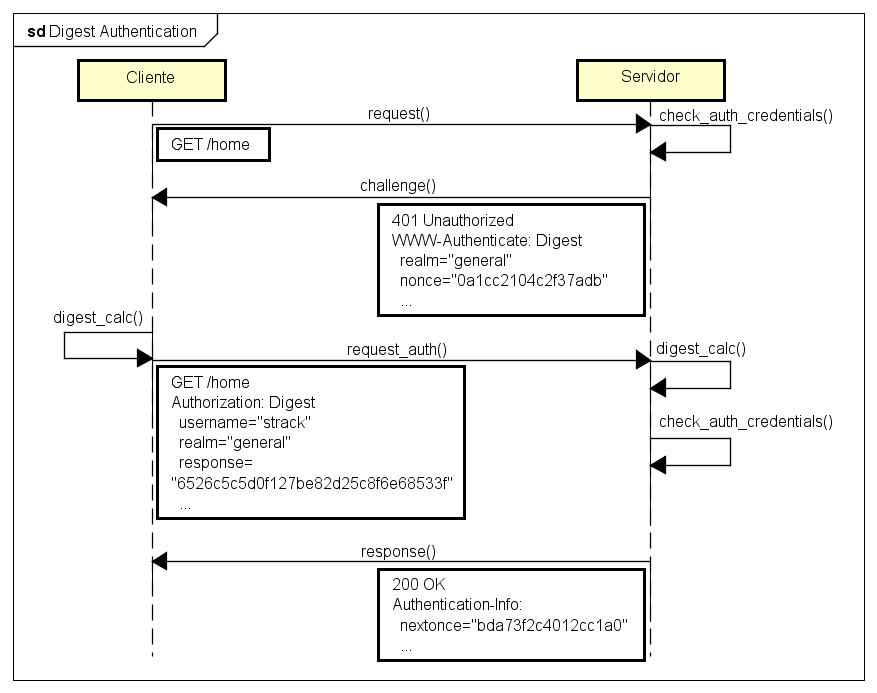
\includegraphics[width=.8\textwidth]{Digest Authentication (Simplified).png}
  \caption{Exemplo de autenticação \emph{Digest}}
  \label{fig:digestAuth}
\end{figure}

\subsection{Autenticação Baseada em Sessão}

Uma sessão web é uma troca de informações semipermanente entre um cliente e um servidor web 
\cite{CALZAVARA2017}. O mecanismo de gerenciamento de estados para o HTTP, baseado em sessões, foi 
especificado na RFC 2109 \cite{RFC2109} com sua versão mais atual especificada na RFC 6265 
\cite{RFC6265}. Este mecanismo utiliza o termo \emph{cookie} para se referir às informações de 
estados que são passadas entre o servidor e o cliente, e salvas no cliente \cite{RFC2109}. 

A autenticação baseada em sessão é o método mais comum de autenticação em sistemas web. Neste 
método, após o envio de credenciais de acesso e validação do usuário por meio de uma requisição 
HTTP, o servidor gera um \emph{cookie}, armazena-o e envia-o pelo cabeçalho \texttt{Set-Cookie} da 
resposta para o cliente. O cliente salva o valor, que é enviado no cabeçalho \texttt{Cookie} em 
toda requisição para o mesmo servidor de origem \cite{PAPATHANASAKI2022} (Figura \ref{fig:sessionAuth}).

\begin{figure}[ht]
  \centering
  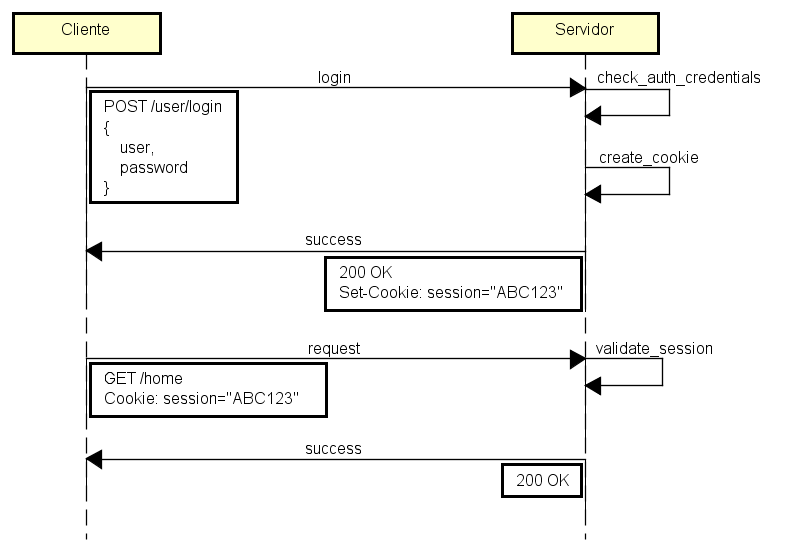
\includegraphics[width=.8\textwidth]{Session-Based Authentication.png}
  \caption{Exemplo de Autenticação baseada em sessão}
  \label{fig:sessionAuth}
\end{figure}

\subsection{Autenticação Baseada em Token}

\emph{Tokens} são itens utilizados para identificar e autenticar usuários. São palavras assinadas e 
não criptografadas, que carregam informações sobre um usuário autenticado \cite{BALAJ2017}. O 
padrão mais utilizado deste tipo de autenticação é o JSON \emph{Web Token} (JWT), que foi proposto
na RFC 7519. O JWT é um formato compacto de representação de reinvindicações (\emph{claims}), 
destinado a ambientes com restrição de espaço, como cabeçalhos HTTP e parâmetros de consulta de URI 
(\emph{Uniform Resource Identifier}) \cite{RFC7519}.

Um JSON \emph{Web Token} é composto por cadeias de caracteres codificadas em \emph{base64url} (codificação
\emph{base64} com alterações para uso em URLs e nomes de arquivo), separadas 
por ponto. Geralmente possuem 3 cadeias: o cabeçalho, que contém informações a respeito do tipo de mídia do 
JWT e da criptografia usada para assinar o \emph{token}; a carga útil (\emph{payload}), que contém 
as informações sobre as \emph{claims}, que são conjuntos de declarações sobre uma entidade 
(geralmente um usuário); e a assinatura, que é a concatenação dos \emph{hashes} gerados a partir das 
outras duas cadeias com uma chave secreta ou certificado, utilizada para verificação de integridade
do \emph{token} \cite{MONTANHEIRO2017}.

Neste método, após o envio de credenciais de acesso e validação do usuário por meio de uma 
requisição HTTP, o servidor gera um \emph{token}, que é enviado para o cliente e pode ser salvo
em \emph{cookies} ou no armazenamento local \cite{MONTANHEIRO2017}. Também pode ser enviado um 
\emph{token} de atualização (\emph{refresh token}), para a obtenção de um novo \emph{token} de acesso
assim que o atual expirar. Ao possuir o \emph{token}, quando uma requisição é feita ao servidor o 
mesmo deve ser enviado no cabeçalho \texttt{Authorization}, precedido pela palavra \emph{Bearer}. 
\cite{RFC6749} (Figura \ref{fig:tokenAuth}).

\begin{figure}[ht]
  \centering
  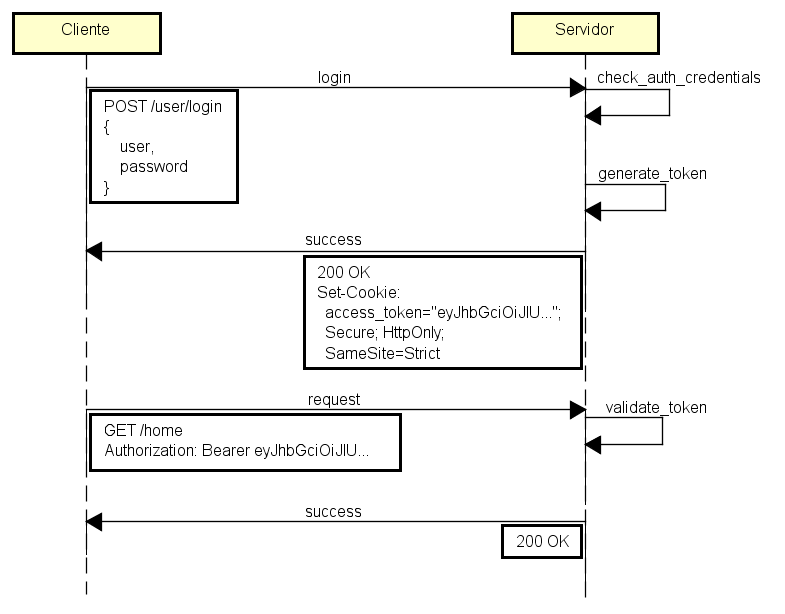
\includegraphics[width=.85\textwidth]{Token-Based Authentication.png}
  \caption{Exemplo de Autenticação baseada em \emph{token}.}
  \label{fig:tokenAuth}
\end{figure}

\

\
\
\subsection{OAuth e OAuth2}
\
\subsection{OpenID}
\
\section{Materiais e Métodos}


\
\section{Resultados e Discussão}
\
\section{Conclusão}
\
% \section{First Page} \label{sec:firstpage}

% The first page must display the paper title, the name and address of the
% authors, the abstract in English and ``resumo'' in Portuguese (``resumos'' are
% required only for papers written in Portuguese). The title must be centered
% over the whole page, in 16 point boldface font and with 12 points of space
% before itself. Author names must be centered in 12 point font, bold, all of
% them disposed in the same line, separated by commas and with 12 points of
% space after the title. Addresses must be centered in 12 point font, also with
% 12 points of space after the authors' names. E-mail addresses should be
% written using font Courier New, 10 point nominal size, with 6 points of space
% before and 6 points of space after.

% The abstract and ``resumo'' (if is the case) must be in 12 point Times font,
% indented 0.8cm on both sides. The word \textbf{Abstract} and \textbf{Resumo},
% should be written in boldface and must precede the text.

% \section{CD-ROMs and Printed Proceedings}

% In some conferences, the papers are published on CD-ROM while only the
% abstract is published in the printed Proceedings. In this case, authors are
% invited to prepare two final versions of the paper. One, complete, to be
% published on the CD and the other, containing only the first page, with
% abstract and ``resumo'' (for papers in Portuguese).

% \section{Sections and Paragraphs}

% Section titles must be in boldface, 13pt, flush left. There should be an extra
% 12 pt of space before each title. Section numbering is optional. The first
% paragraph of each section should not be indented, while the first lines of
% subsequent paragraphs should be indented by 1.27 cm.

% \subsection{Subsections}

% The subsection titles must be in boldface, 12pt, flush left.

% \section{Figures and Captions}\label{sec:figs}


% Figure and table captions should be centered if less than one line, otherwise justified and 
% indented by 0.8cm on
% both margins, as shown in Figure. The caption font must
% be Helvetica, 10 point, boldface, with 6 points of space before and after each
% caption.


% In tables, try to avoid the use of colored or shaded backgrounds, and avoid
% thick, doubled, or unnecessary framing lines. When reporting empirical data,
% do not use more decimal digits than warranted by their precision and
% reproducibility. Table caption must be placed before the table (see Table 1)
% and the font used must also be Helvetica, 10 point, boldface, with 6 points of
% space before and after each caption.

% \section{Images}

% All images and illustrations should be in black-and-white, or gray tones,
% excepting for the papers that will be electronically available (on CD-ROMs,
% internet, etc.). The image resolution on paper should be about 600 dpi for
% black-and-white images, and 150-300 dpi for grayscale images.  Do not include
% images with excessive resolution, as they may take hours to print, without any
% visible difference in the result. 

% \section{References}


% The references must be listed using 12 point font size, with 6 points of space
% before each reference. The first line of each reference should not be
% indented, while the subsequent should be indented by 0.5 cm.

\bibliographystyle{sbc}
\bibliography{references}

\end{document}
